\section{Annexes}

\subsection{Rapport détaillé du test de charge Gatling sur MF Banking}

\begin{figure}[h!]
	\centering
		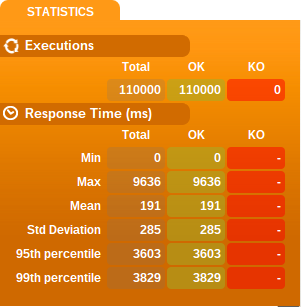
\includegraphics[scale=0.5]{global.png}
	\caption{Stastiques globales du test : nombre de requêtes réussies et echouées et détails du temps de réponse}
\end{figure}

\begin{figure}[h!]
	\centering
		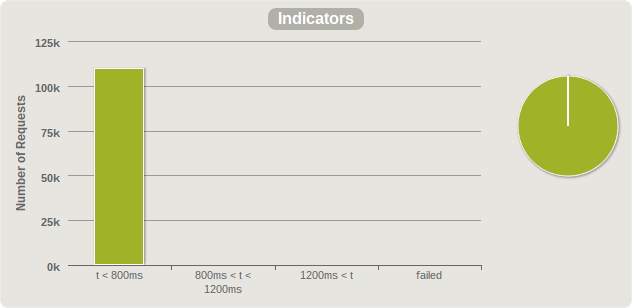
\includegraphics[scale=0.5]{indicators.png}
	\caption{On peut voir que presque toutes les requêtes ont été effectués en moins de 800 ms}
\end{figure}

\begin{figure}[h!]
	\centering
		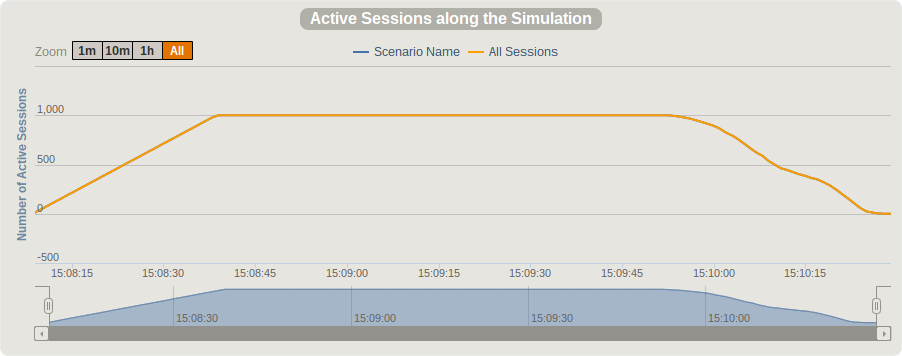
\includegraphics[scale=0.5]{active-sessions.png}
	\caption{Nombres d'utilisateurs actifs simultanement. La montée progressive du nombres d'utilisateurs au début est dû à une \textit{rampe} : on demande à Gatling de prendre 30 secondes pour lancer progressivement les 1000 utilisateurs du test}
\end{figure}

\begin{figure}[h!]
	\centering
		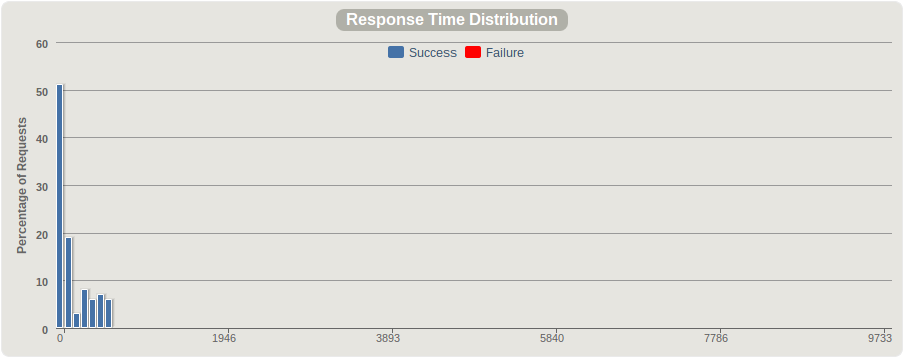
\includegraphics[scale=0.5]{response-time.png}
	\caption{Distribution du temps de réponse : on peut voir que la majorité des requêtes ont été été effectués quasi instantanément et que le nombre de requêtes lentes est tellement faible qu'elles n'apparaissent même pas sur le graphe}
\end{figure}

\begin{figure}[h!]
	\centering
		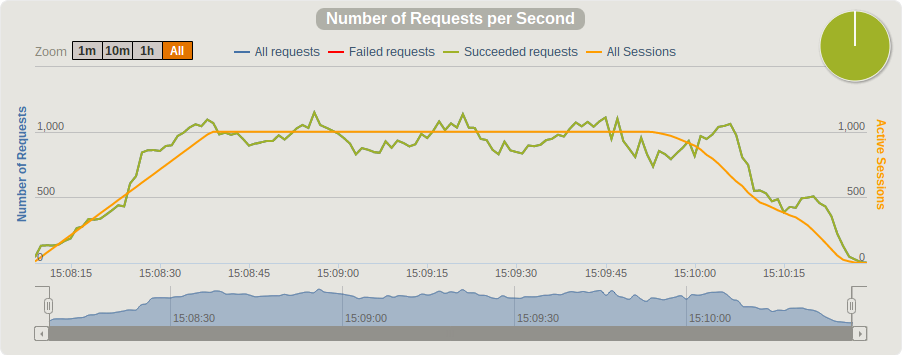
\includegraphics[scale=0.5]{requests.png}
	\caption{Nombre de requêtes qui démarrent par seconde : on observe qu'une fois la rampe terminée, le système se maintient sans difficulté entre 800 et 1200 requêtes par seconde}
\end{figure}

\begin{figure}[h!]
	\centering
		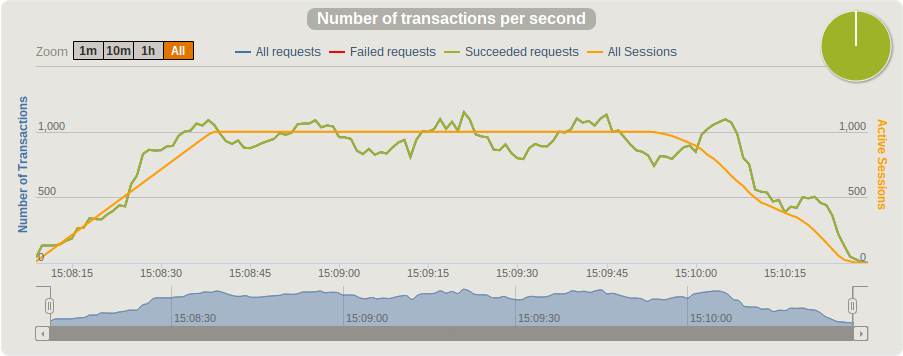
\includegraphics[scale=0.5]{transactions.png}
	\caption{Nombre de transactions (requêtes qui s'achèvent) par seconde : mêmes observations que pour les requêtes, le système se maintient durant tout le test entre 800 et 1200 transactions par seconde}
\end{figure}